\documentclass[manual-fr.tex]{subfiles}
\begin{document}

When the workflow and the training files are selected, click on the button \emph{train SEM} as shown on figure \ref{fig:train_sem-03}. It will open the window allowing to set the parameters of the CRF to retrain SEM, as shown in figure \ref{fig:train_sem-03}. In this window, it is also possible to select a pattern file to train Wapiti. If none are selected, it will be automatically generated from the entries and features computed in the workflow. When all parameters are configured, click on the \emph{train} button to launch the training of a new SEM model. When the training is finished, SEM will display where files are located on the computer, as shown in the figure \ref{fig:train_sem-06}. To use the model, copy the file \emph{model.txt} in the folder \emph{\$\{SEM\_DATA\}/resources/models/fr/NER}.

\begin{figure}[ht!]
    \begin{center}
    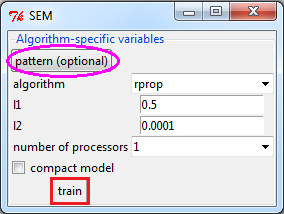
\includegraphics[scale=0.75]{fr/images/train_sem-05.png}
    \end{center}
    \caption{Circled in purple: the button to select a model. Framed in red: the button to launch the training.}
    \label{fig:train_sem-05}
\end{figure}

\begin{figure}[ht!]
    \begin{center}
    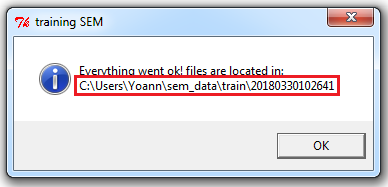
\includegraphics[scale=0.75]{fr/images/train_sem-06.png}
    \end{center}
    \caption{Framed in red : the path where to find the files on the computer.}
    \label{fig:train_sem-06}
\end{figure}

\end{document}
